\documentclass{article} %Classe del documento
\usepackage{float}  %Permette di posizionare le immagini dove si vuole
\usepackage{booktabs} %Permette di creare tabelle con linee orizzontali
\usepackage[svgnames]{xcolor} %Permette di usare i colori
\usepackage{listings} %Permette di inserire codice R nel documento
\usepackage{upquote} %Permette di usare i singoli apici
\usepackage{graphicx} %Permette di inserire immagini
\usepackage{verbatim} %Permette di inserire commenti multiriga
\usepackage[a4paper, left=1.60in, right=1.60in, top=1.7in, bottom=1.7in]{geometry}
%\usepackage[a4paper, margin=1.6in]{geometry}
\usepackage{changepage} %Permette di regolare i margini
\usepackage[utf8]{inputenc} %Permette l'uso dei caratteri accentati
\usepackage[italian]{babel} %Permette l'uso della la lingua italiana
\usepackage{setspace}
\usepackage{graphicx}
\usepackage{tabularx}
\usepackage{caption}
% \title{\texttt{Mussels}}
% \author{Stefano Terrone e Leonardo Perin}
% \date{20 gennaio 2025}

\begin{document}

%Aggiunge spaziatura di 1.5
\onehalfspacing

% \maketitle

\newpage
% \begin{flushleft}
%     %\vskip 50pt
% \textbf{\Large 0.1 \: Introduzione}    
% \end{flushleft}

% \vskip 10pt

% \hspace{0.20in}
% il database è composto da \textbf{n} variabili:
% \begin{itemize}
%     \item \texttt{}: 
%     \item \texttt{}: 
%     \item \texttt{}: 
%     \item \texttt{}:  
%     \item \texttt{}: 
%     \item \texttt{}:
%     \item \texttt{}:
% \end{itemize}
% Le analisi sono state eseguite con il software R nella versione 4.2.3.\\ Il livello di significatività è fissato al 5\%.
% \vskip 55pt 

\newpage
\begin{flushleft}
    %\vskip 30pt
    \textbf{\Huge 1. \: Analisi esplorative}
    \vskip 30pt
    %Prima parte: analisi univariate
    %Titolo
    \textbf{\Large 1.1 \: Analisi Univariate}
\end{flushleft}
\vskip 10pt

%Introduzioni analisi esplorative
Il database è composto da 44 osservazioni, una per ciascun fiume, e 9 varabili. Le varabili rappresentano varie caratteristiche dei fiumi come il numero di specie di cozze presenti, la dimensione del fiume, la distanza da alcuni fiumi importanti, e vari indicatori sulla qualità delle acque.\\

%Tabella di sintesi
\begin{table}[H]
    \centering
    \renewcommand{\arraystretch}{1.4} % Increases the row height
    \begin{tabularx}{\textwidth}{p{69pt}l p{30pt}c p{45pt}c p{35pt}c p{40pt}c p{30pt}c p{27pt}r}
        \toprule
        & Min. & 1\textsuperscript{0} qt. & Mediana(IQR) & Media(sd) & 3\textsuperscript{0} qt. & Max\\
            \midrule  
            \texttt{Species} & 2.00 & 8.00 & 10.00(5.0) & 11.25(5.99) & 13.00 & 33.00 \\
            \texttt{Area} & 349 & 2115 & 4315(7797.5) & 6590(6016) & 9912 & 27900 \\
            \texttt{Stepping}\\ \texttt{stones to AC} & 1.00 & 7.00 & 15.50(15.25) & 15.34(9.19) & 22.25 & 33.00 \\
            \texttt{Stepping }\\
            \texttt{stones to AP} & 0.00 & 4.00 & 12.00(14.25) & 12.02(8.24) & 18.25 & 28.00 \\
            \texttt{Stepping }\\
            \texttt{stones to SV} & 0.00 & 5.00 & 7.00(13.25) & 8.136(8.94) & 11.00 & 21.00 \\
            \texttt{Stepping }\\
            \texttt{stones to SL} & 4.00 & 16.75 & 22.00(0.775) & 22.16(1.84) & 30.00 & 36.00 \\
            \texttt{Nitrate} & 0.100 & 0.600 & 0.800(0.775) & 1.495(1.84) & 1.375 & 8.700 \\
            \texttt{Solid Residue} & 29.0 & 56.5 & 78.0(64.0) & 112.4(17.3) & 120.5 & 520.0 \\
            \texttt{Hydronium} & 0.200 & 1.00 & 1.600(2.2) & 3.631(6.03) & 3.200 & 32.00 \\
            \texttt{ln(Area)} & 5.855 & 7.657 & 8.370(1.54) & 8.331(1.07) & 9.201 & 10.24 \\
        \bottomrule
    \end{tabularx}
    \caption{Tabella di sintesi}
\end{table}
%Introduzione analisi univariate

%Esempio di analisi univariata su una variabile
%Titolo
% \newpage
% \begin{center}
% \textbf{\large }
% \end{center}

%Grafico delle variabili univariate
% \begin{figure}[H]
%     \centering
%     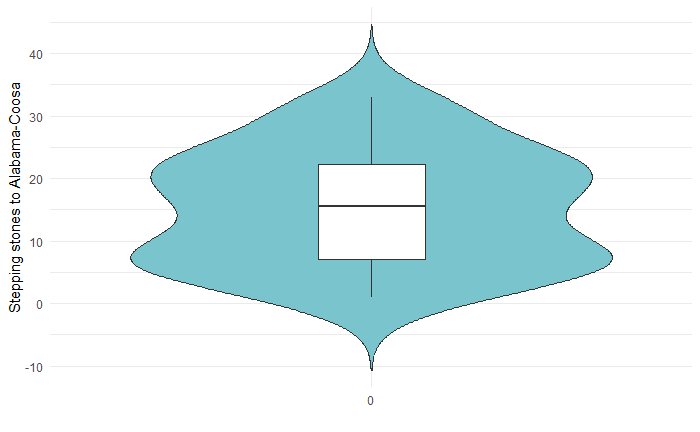
\includegraphics[width=0.6\textwidth]{immagini/vp_ac.png}
%     \caption{}
% \end{figure}

% \begin{figure}[H]
%     \centering
%     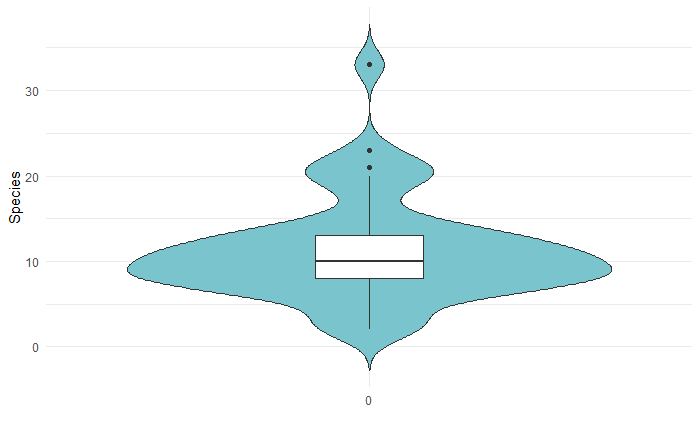
\includegraphics[width=0.47\textwidth]{immagini/vp_species.png}
%     \hspace{0.04\textwidth}% Distanza tra le immagini
%     \includegraphics[width=0.47\textwidth]{C:/Users/Stefa/Documents/1-Stefano/1-Medica/Lab10/grafici/4.png}
%     \caption{A sinistra: curve di sopravvivenza di Kaplan-Meier.\\ A destra: curve di sopravvivenza basato sulla trasformazione complementare del logaritmo log-log.}
% \end{figure}

\begin{figure}[H]
    \centering
    \begin{minipage}{0.49\textwidth}
        \centering
        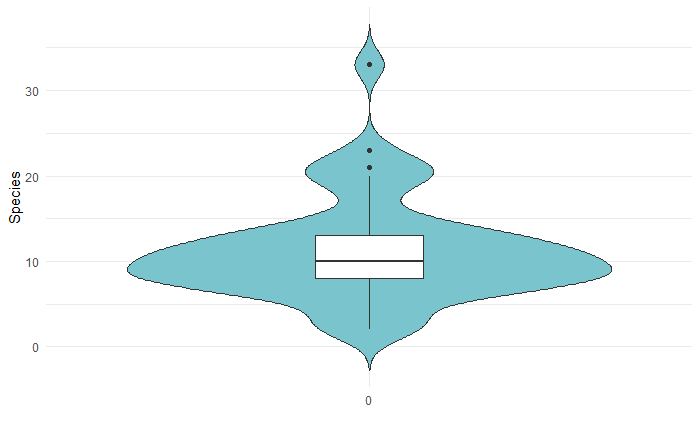
\includegraphics[width=\textwidth]{immagini/vp_species.png}
        \captionsetup{justification=centering}
        \caption{Violinplot della variabile \texttt{species}}
    \end{minipage}
    \hfill
    \begin{minipage}{0.49\textwidth}
        \centering
        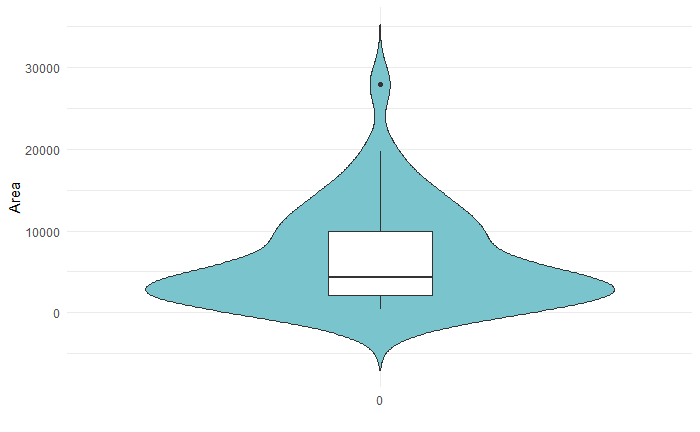
\includegraphics[width=\textwidth]{immagini/vp_area.png}
        \captionsetup{justification=centering}
        \caption{Violinplot della variabile\\ \texttt{Area}}
    \end{minipage}
\end{figure}
La variabile \texttt{Species}, rappresentante il numero di specie di cozze nel fiume, ha una distribuzione asimmetrica a destra come evidenziato dal violinplot \textit{(Figura 1)}. Ha un valore minimo di 2 specie (nel fiume Waccasassa) e un massimo di 33 specie (nel fiume Apalachicola). La mediana è di 10 specie, la media è di 11.25 specie.
La variabile \texttt{Area} segue una distribuzione asimmetrica a destra \textit{(Figura 2)}, con un valore minimo di 349 sq mi \textit{(square mile)} e un massimo di 27900 sq mi. La mediana è di 4315 sq mi, la media è di 6590 sq mi \textit{(Tabella 1)}.

\begin{figure}[H]
    \centering
    \begin{minipage}{0.49\textwidth}
        \centering
        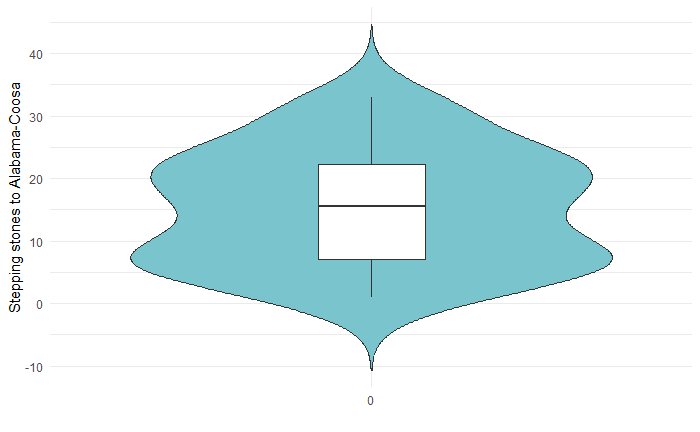
\includegraphics[width=\textwidth]{immagini/vp_ac.png}
        \captionsetup{justification=centering}
        \caption{Violinplot della variabile \texttt{stepping stones to AC}}
    \end{minipage}
    \hfill
    \begin{minipage}{0.49\textwidth}
        \centering
        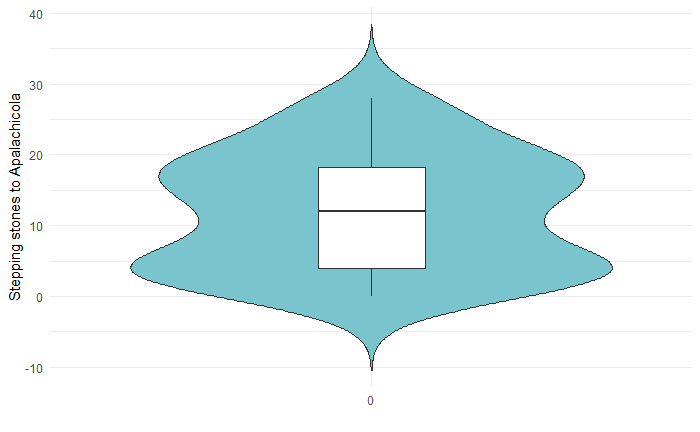
\includegraphics[width=\textwidth]{immagini/vp_ap.png}
        \captionsetup{justification=centering}
        \caption{Violinplot della variabile \texttt{stepping stones to AP}}
    \end{minipage}
\end{figure}
La distanza dal sistema fluviale di Alabama-Coose (\texttt{Stepping stones to AC}) segue una distribuzione simmetrica \textit{(Figura 3)}, suggerendo che i fiumi sono equamente distribuiti rispetto a questo sistema fluviale. La distanza minima è di 1 e la massima di 33. La idstanza media è di 15.34, e quella mediana di 15.50 "saltelli".
Anche la distanza dal fiume Apalachicola (\texttt{Stepping stones to AP}) segue una distribuzione simmetrica \textit{(Figura 4)}, con una distanza minima di 0 (coincidente con il fiume stesso) e una massima di 28. La distanza media è di 12.02, e quella mediana di 12.00 "saltelli" \textit{(Tabella 1)}.

\begin{figure}[H]
    \centering
    \begin{minipage}{0.49\textwidth}
        \centering
        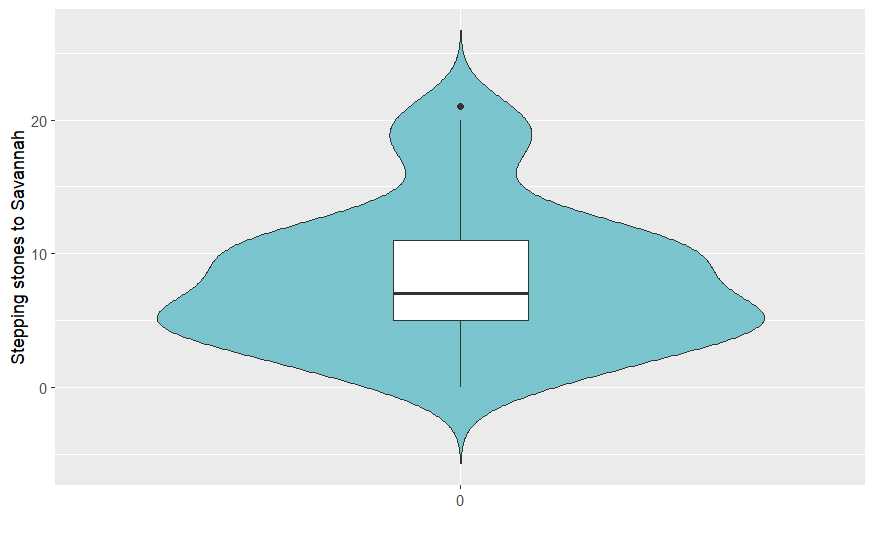
\includegraphics[width=\textwidth]{immagini/vp_sv.png}
        \captionsetup{justification=centering}
        \caption{Violinplot della variabile \texttt{stepping stones to SV}}
    \end{minipage}
    \hfill
    \begin{minipage}{0.49\textwidth}
        \centering
        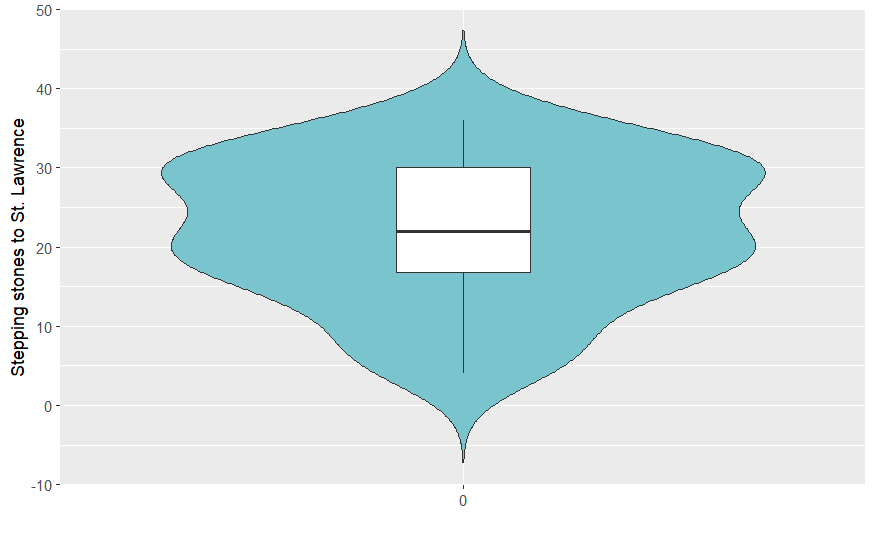
\includegraphics[width=\textwidth]{immagini/vp_sl.png}
        \captionsetup{justification=centering}
        \caption{Violinplot della variabile \texttt{stepping stones to SL}}
    \end{minipage}
\end{figure}
La distanza dal fiume Savannah (\texttt{Stepping stones to SV}) ha una distribuzione simmetrica anche se presenta una leggera coda lunga a destra \textit{(Figura 5)}, con una distanza minima di 0 (coincidente con il fiume stesso) e una massima di 21. La distanza media è di 8.136, e quella mediana di 7.00. Il valore molto basso della mediana e la presenza di una piccola coda lunga a destra suggeriscono che la maggior parte dei fiumi osservati sono molto vicini al fiume Savannah.
La distanza dal fiume St.\ Lawrence (\texttt{Stepping stones to SL}) ha una distribuzione simmetrica \textit{(Figura 6)}, ma presenta anche una leggera coda lunga a sinistra. La distanza minima di 4 e una massima di 36. La distanza media è di 22.16, e quella mediana di 22.00. Il valore elevato della di media e mediana, in aggiunta alla leggera coda a sinistra, suggerisce che la maggior parte dei fiumi sono distanti al fiume St. Lawrence \textit{(Tabella 1)}.


\begin{figure}[H]
    \centering
    \begin{minipage}{0.49\textwidth}
        \centering
        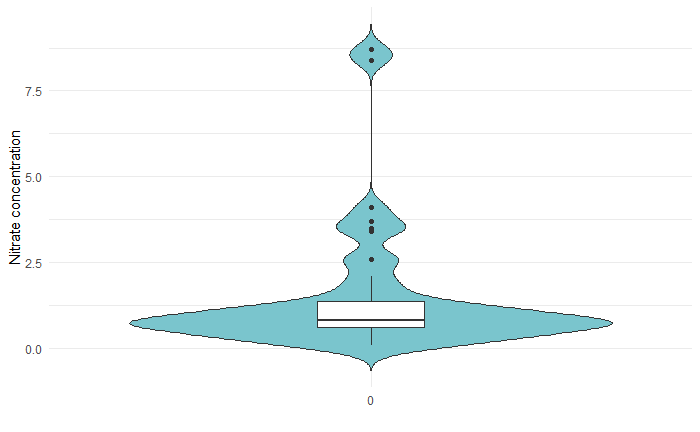
\includegraphics[width=\textwidth]{immagini/vp_nitrate.png}
        \captionsetup{justification=centering}
        \caption{Violinplot della variabile \texttt{Nitrate}}
    \end{minipage}
    \hfill
    \begin{minipage}{0.49\textwidth}
        \centering
        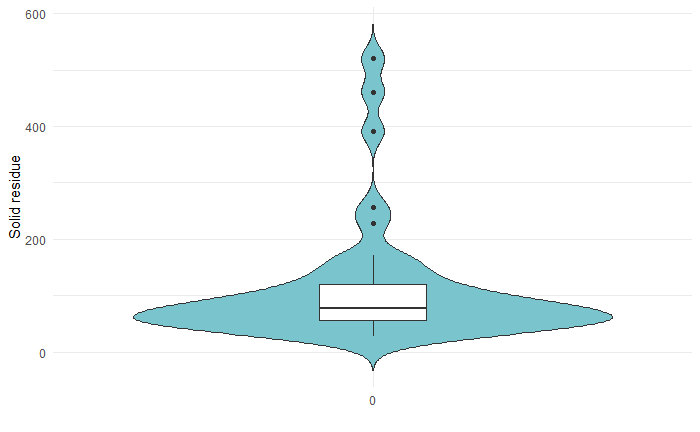
\includegraphics[width=\textwidth]{immagini/vp_sd.png}
        \captionsetup{justification=centering}
        \caption{Violinplot della variabile \texttt{solid residue}}
    \end{minipage}
\end{figure}
La variabile \texttt{Nitrate} ha una distribuzione asimmetrica a destra \textit{(Figura 7)}, con un valore minimo di 0.100 ppm \textit{(parts per million)} e un massimo di 8.700 ppm. La mediana è di 0.800 ppm, la media è di 1.495 ppm.
la variabile \texttt{Solid Residue} ha anche essa una distribuzione asimmetrica a destra \textit{(Figura 8)}, con un valore minimo di 29.0 ppm e un massimo di 520.0 ppm. La mediana è di 78.0 ppm, la media è di 112.4 ppm \textit{(Tabella 1)}.


\begin{figure}[H]
    \centering
    \begin{minipage}{0.49\textwidth}
        \centering
        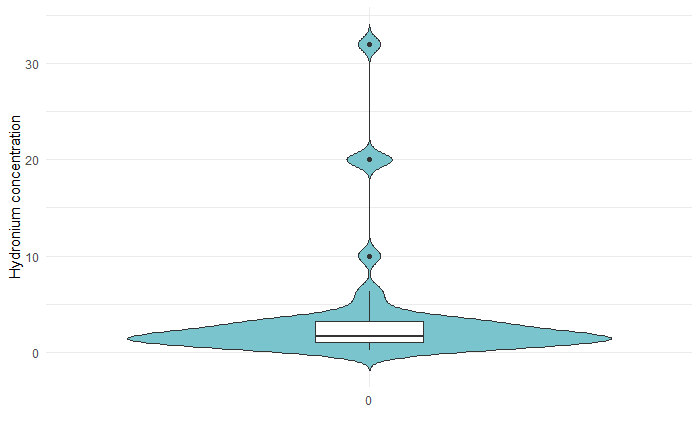
\includegraphics[width=\textwidth]{immagini/vp_hy.png}
        \captionsetup{justification=centering}
        \caption{Violinplot della variabile \texttt{hydronium}}
    \end{minipage}
    \hfill
    \begin{minipage}{0.49\textwidth}
        \centering
        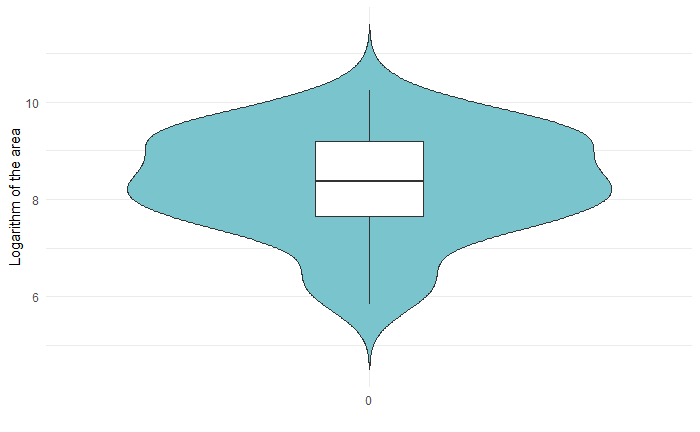
\includegraphics[width=\textwidth]{immagini/vp_ln.png}
        \captionsetup{justification=centering}
        \caption{Violinplot della variabile \texttt{ln(Area)}}
    \end{minipage}
\end{figure}
La variabile \texttt{Hydronium} ha una distribuzione asimmetrica a destra \textit{(Figura 9)}, con un valore minimo di 0.200 e un massimo di 32.00. La mediana è di 1.600, la media è di 3.631.
La variabile \texttt{ln(Area)} segue una distribuzione simmetrica \textit{(Figura 10)}, con un valore minimo di 5.855 e un massimo di 10.24. La mediana è di 8.370, la media è di 8.331 \textit{(Tabella 1)}.


%Seconda parte: analisi bivariate
%Titolo
\newpage
\begin{flushleft}
    
    \textbf{\Large 1.2 \: Analisi Bivariate}
    \vskip 10pt
\end{flushleft}
\vskip 10pt

%Introduzione analisi bivariate
Si valuta la relazione tra le varie variabili. Delle 35 bivariate totali, 17 bivaraite sono risultate significative \textit{(Tabella 2)}.\\

\end{document}

% \begin{figure}[H]
%     \centering
%     \begin{minipage}{0.30\textwidth}
%         \centering
%         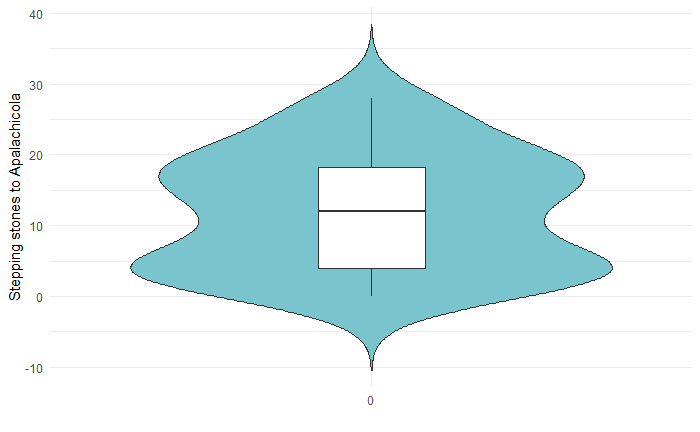
\includegraphics[width=\textwidth]{immagini/vp_ap.png}
%         \captionsetup{justification=centering}
%         \caption{Violinplot della variabile \texttt{stepping stones to AP}}
%     \end{minipage}
%     \hfill
%     \begin{minipage}{0.30\textwidth}
%         \centering
%         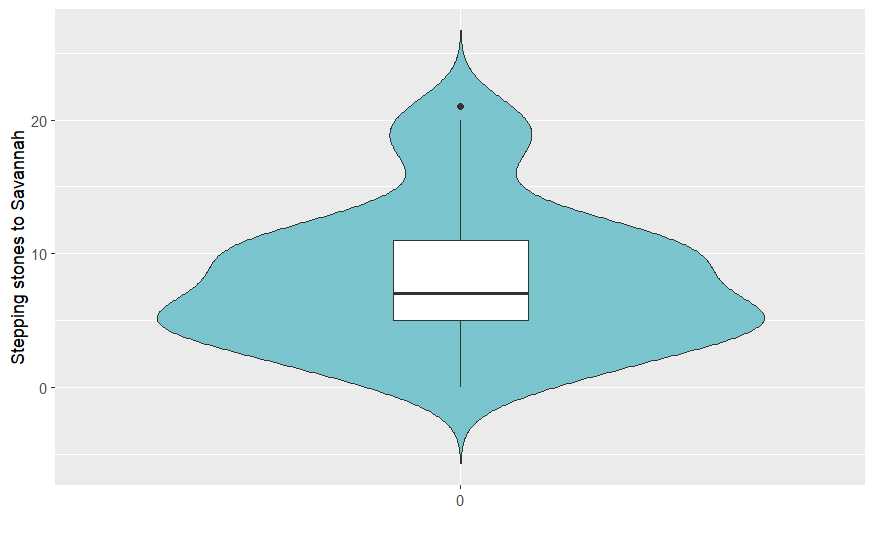
\includegraphics[width=\textwidth]{immagini/vp_sv.png}
%         \captionsetup{justification=centering}
%         \caption{Violinplot della variabile \texttt{stepping stones to SV}}
%     \end{minipage}
%     \hfill
%     \begin{minipage}{0.30\textwidth}
%         \centering
%         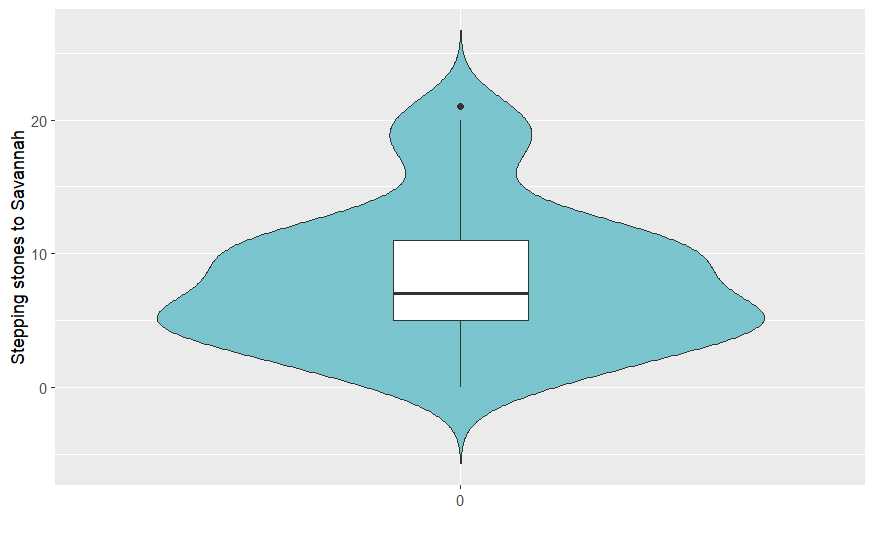
\includegraphics[width=\textwidth]{immagini/vp_sv.png}
%         \captionsetup{justification=centering}
%         \caption{Violinplot della variabile \texttt{stepping stones to SV}}
%     \end{minipage}
% \end{figure}